\chapter{Conception Mécanique et Électronique}
\label{ch:mecanique}

\section{Architecture différentielle}
\label{sec:meca_diff}

\esibot{} adopte une architecture \emph{differential drive}~: deux roues motrices
indépendantes plus une roue folle assurant la stabilité statique, la direction résultant
uniquement de la différence de vitesse entre les deux roues. Les fichiers \gls{cad}/STL du
châssis constituent un livrable séparé (Livrable~1) non inclus dans le code analysé~; ce
chapitre s'appuie donc sur le modèle \gls{urdf} (\texttt{esibot\_description}), source de
vérité utilisée par \ros{} pour les transformées et les costmaps, complété par les
constantes électroniques relevées dans le code de commande.

\section{Modèle géométrique}
\label{sec:meca_urdf}

\begin{table}[H]
	\centering
	\caption{Paramètres géométriques et inertiels déclarés dans le modèle \gls{urdf}.}
	\label{tab:urdf_geom}
	\begin{tabularx}{\linewidth}{L{5cm} C{3.2cm} L{5cm}}
		\toprule
		\textbf{Élément} & \textbf{Valeur} & \textbf{Remarque} \\
		\midrule
		Châssis (\texttt{base\_link}) & 0.21 $\times$ 0.14 $\times$ 0.03\,m & masse 2.0\,kg \\
		Rayon de roue (\texttt{wheel\_radius}) & 0.025\,m & largeur 0.027\,m, masse 0.2\,kg/roue \\
		Empattement (\texttt{wheel\_y} $\times 2$) & 0.14\,m & distance latérale entre roues \\
		Module caméra (\texttt{camera\_link}) & 0.073 $\times$ 0.278 $\times$ 0.073\,m & masse 0.56\,kg, $x=-0.105$\,m (arrière) \\
		\bottomrule
	\end{tabularx}
\end{table}

Le modèle déclare les repères optiques caméra (\texttt{camera\_depth\_frame},
\texttt{camera\_rgb\_optical\_frame}, rotation $-\pi/2$) ; un
\texttt{static\_transform\_publisher} relie \texttt{camera\_depth\_frame} au repère natif
du pilote Kinect \texttt{kinect\_depth} par une transformée identité.

\begin{warnbox}
	Une révision des paramètres géométriques (notamment le rayon des roues et l'empattement) est nécessaire pour garantir une parfaite cohérence entre le modèle \gls{urdf} et le code de commande bas-niveau, afin d'optimiser la précision de l'odométrie.
\end{warnbox}

\section{Cinématique différentielle et odométrie}
\label{sec:meca_kinematics}

La conversion \topic{/cmd\_vel} $\to$ vitesses de roue, implémentée dans
\texttt{motor\_bridge\_node.py} (\texttt{twist\_to\_wheel\_\allowbreak commands}) et répliquée dans le
tableau de bord (\texttt{imu\_web\_dashboard.py}), suit le modèle classique~:

\begin{equation}
	v_{\text{g}} = v - \omega \cdot \tfrac{L}{2}, \quad
	v_{\text{d}} = v + \omega \cdot \tfrac{L}{2}
	\label{eq:diff_drive}
\end{equation}

et inversement pour la reconstruction d'odométrie~:
$v = (v_{\text{g}}+v_{\text{d}})/2$, $\omega = (v_{\text{d}}-v_{\text{g}})/L$
(équation~\ref{eq:diff_drive_inverse}), où $L$ est l'empattement.
\begin{equation}
	v = \frac{v_{\text{g}} + v_{\text{d}}}{2}, \qquad
	\omega = \frac{v_{\text{d}} - v_{\text{g}}}{L}
	\label{eq:diff_drive_inverse}
\end{equation}

\begin{figure}[H]
	\centering
	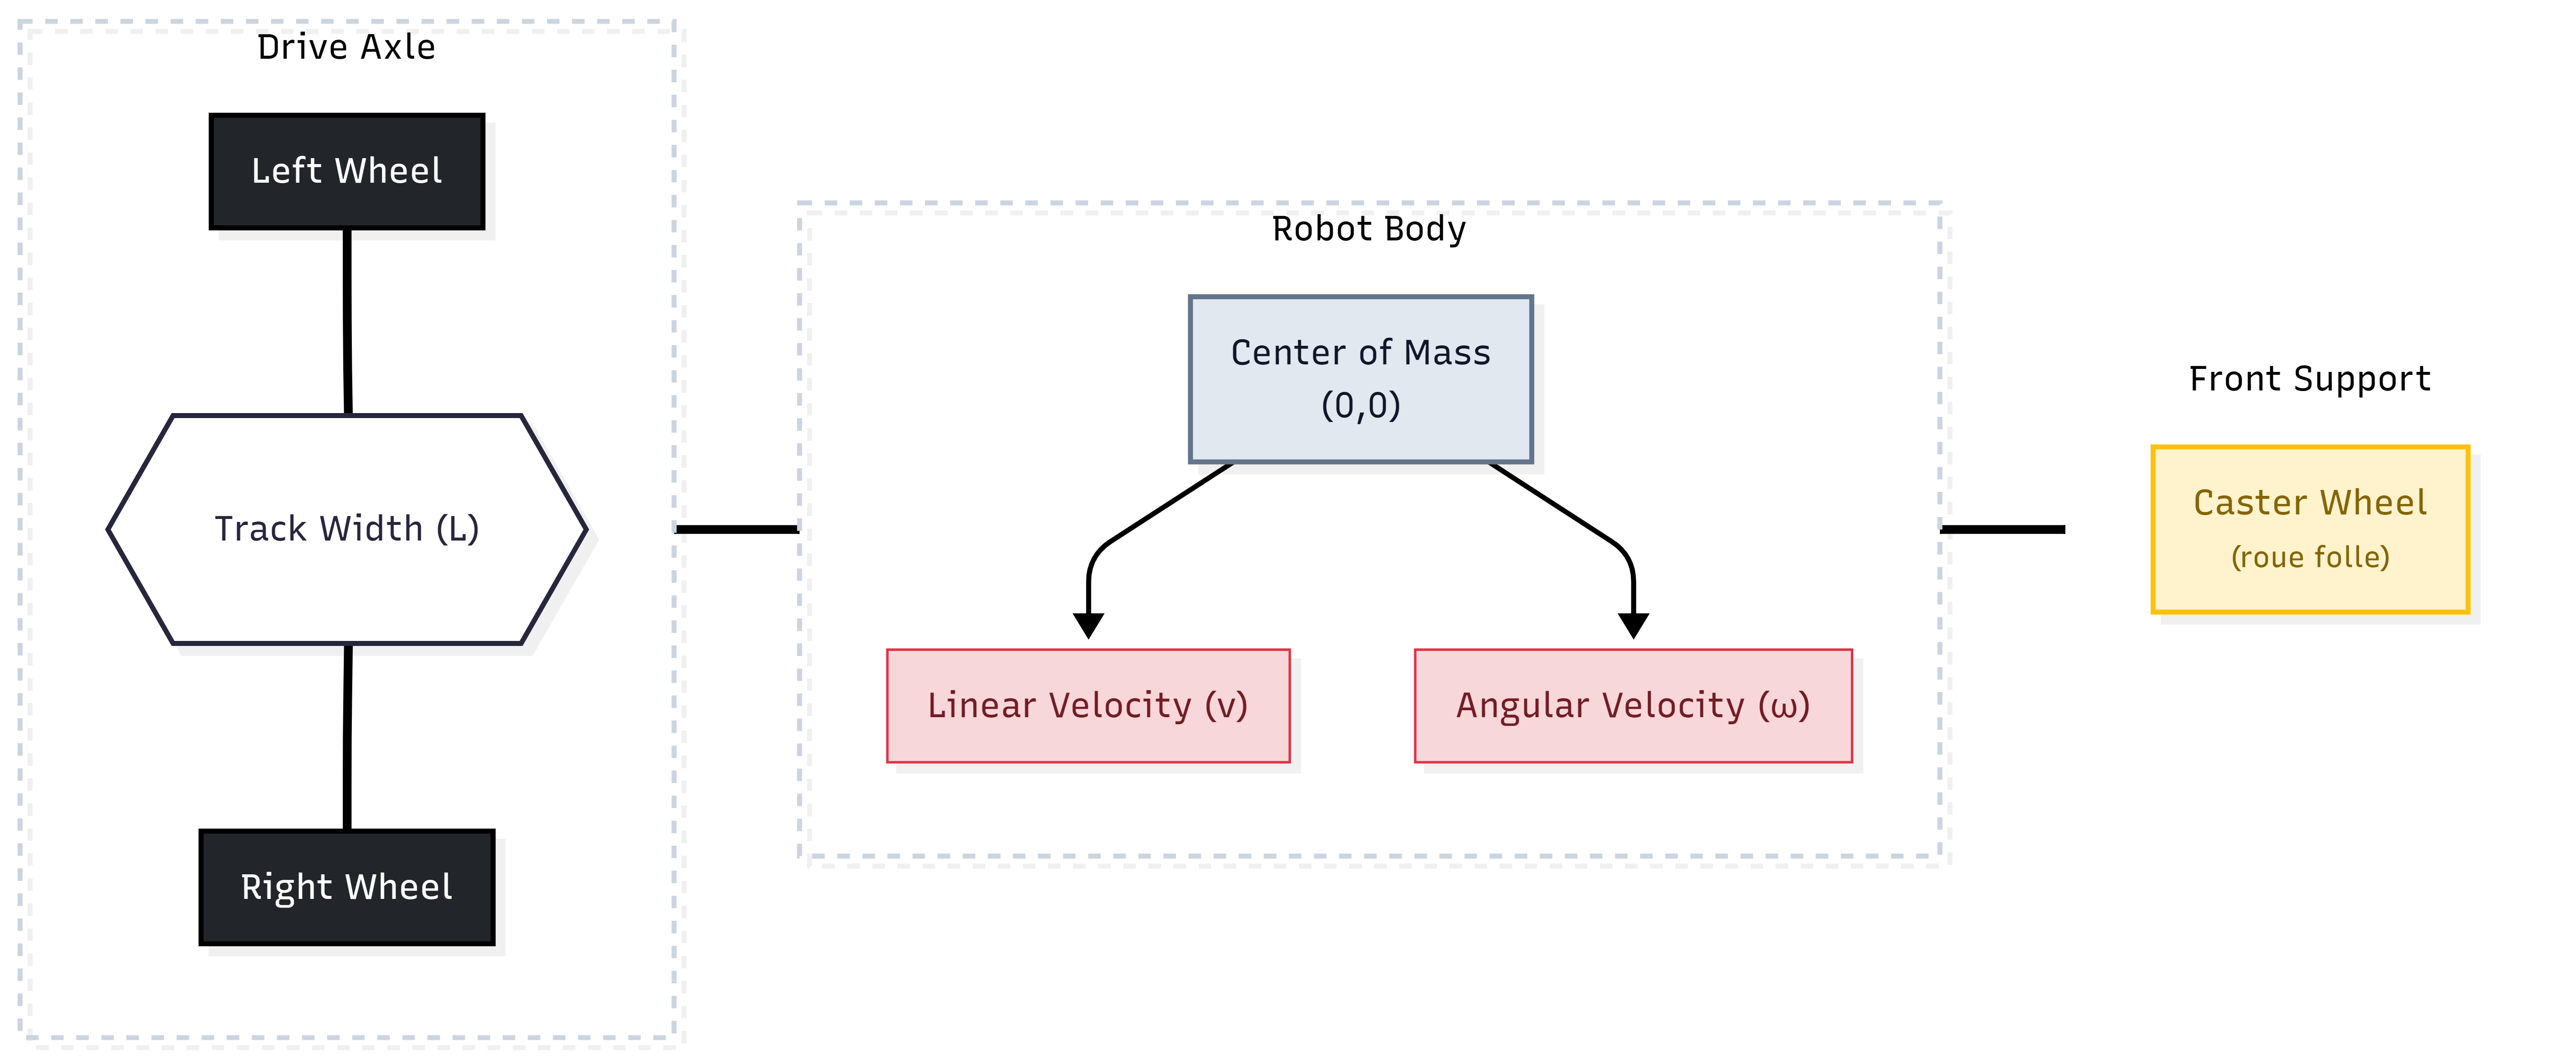
\includegraphics[width=0.5\linewidth]{images/diff_drive_diagram.png}
	\caption{Modèle cinématique du robot différentiel \esibot{} (vue de dessus).}
	\label{fig:diff_drive_diagram}
\end{figure}

Chaque roue est équipée d'un encodeur compté par interruption \gls{gpio}, anti-rebond
logiciel 2\,ms. Le paramètre \texttt{encoder\_cpr} (12 par défaut) est doublé par comptage
sur les deux fronts (\texttt{encoder\_count\_both\_\allowbreak edges=True}), donnant
\textbf{24 impulsions/tour}. La vitesse de rotation mesurée est calculée à chaque cycle de
contrôle (\texttt{control\_hz}, 10\,Hz par défaut) par~:
\begin{equation}
	\text{RPM}_{\text{mesuré}} = \frac{N_{\text{impulsions}}}{\text{CPR}_{\text{effectif}}} \times \frac{60}{\Delta t}
	\label{eq:rpm_measure}
\end{equation}
soit $360^\circ/24=15^\circ$ par impulsion et, avec le rayon de 0.033\,m du calibrateur,
$\approx$\textbf{8.6\,mm}/impulsion ($2\pi\times0.033/24$).

\section{Câblage électronique}
\label{ch:electronique}
\label{sec:elec_topology}

Le cahier des charges (Livrable~2) exige un schéma Fritzing/KiCad, absent de l'archive
fournie~; le tableau~\ref{tab:gpio_pinout} a donc été \textbf{reconstruit par
rétro-ingénierie} depuis les constantes \gls{gpio} du code Python. À la différence du
cahier des charges, qui prévoyait que l'ESP32-CAM pilote le pont en H, le servo et le
HC-SR04, l'implémentation réelle concentre toute l'électronique temps-réel sur les broches
\gls{gpio} du Raspberry\,Pi\,4.

\begin{table}[H]
	\centering
	\caption{Broches \gls{gpio} du Raspberry\,Pi\,4 (BCM), reconstruites depuis le code source.}
	\label{tab:gpio_pinout}
	\begin{tabularx}{\linewidth}{L{3.8cm} C{1.6cm} L{6.8cm}}
		\toprule
		\textbf{Fonction} & \textbf{GPIO} & \textbf{Source / nœud} \\
		\midrule
		ENA / IN1 / IN2 (moteur g.) & 12 / 5 / 6 & \texttt{motor\_bridge\_node}, \texttt{motor\_calibrator} \\
		Encodeur gauche & 26 & \texttt{motor\_bridge\_node} (\texttt{pin\_left\_encoder}) \\
		ENB / IN3 / IN4 (moteur d.) & 13 / 21 / 20 & \texttt{motor\_bridge\_node}, \texttt{motor\_calibrator} \\
		Encodeur droit & 27 & \texttt{motor\_bridge\_node} (\texttt{pin\_right\_encoder}) \\
		\gls{i2c} SDA/SCL (bus 1) & 2 / 3 & \texttt{mpu6050\_node} (MPU6050 @ 0x68) \\
		HC-SR04 SIG (trig/écho) & 23 & \texttt{ultrasonic\_scan\_node} (déprécié) \\
		Servo SG90 radar & 18 & \texttt{ultrasonic\_scan\_node} (déprécié) \\
		\bottomrule
	\end{tabularx}
\end{table}

Dans la branche \texttt{working\_build}, le câblage logiciel du calibrateur et celui du
nœud de production sont cohérents~: les deux utilisent les broches BCM~26 et BCM~27 pour
les encodeurs gauche et droit. La calibration PWM$\to$RPM peut donc alimenter directement
\texttt{pwm\_mapper.py}, sous réserve que le rayon de roue et l'empattement utilisés par
l'odométrie soient contrôlés expérimentalement (voir chapitre~\ref{ch:limitations}).

Le pilotage moteur utilise un double pont en H \textbf{L298N} en PWM logiciel
(\texttt{RPi.GPIO}, 500\,Hz), rapport cyclique borné à $[15\,\%,100\,\%]$
(\texttt{min/max\_duty\_cycle}) pour compenser la zone morte mécanique. Le MPU6050
(\gls{i2c} bus~1, adresse \texttt{0x68}) est configuré au démarrage (réveil, diviseur
d'échantillonnage \texttt{SMPLRT\_DIV=0x07}, filtre passe-bas \texttt{DLPF\_CFG=0x03},
$\pm2g$/$\pm250^\circ$/s) et publie à \textbf{50\,Hz}. Le Kinect (v1, ère Xbox\,360), capteur de
cartographie principal, est relié en \textbf{USB} (non \gls{gpio}) et piloté par le paquet
communautaire \texttt{kinect\_ros2} (\texttt{libfreenect}).

\section{Serveur de caméra (ESP32-CAM)}
\label{sec:elec_esp32cam}

Le module ESP32-CAM (\texttt{AI\_THINKER}) sert exclusivement de serveur vidéo \gls{mjpeg}
\gls{wifi}~: le firmware \texttt{CameraServerArduinoIDE.ino} initialise le capteur OV2640
(\texttt{UXGA} si PSRAM, sinon \texttt{SVGA}) et expose le flux sur \texttt{/stream}.
Aucune broche \gls{gpio} de l'ESP32-CAM ne pilote d'actionneur --- l'essentiel de ses
broches étant réservé à l'interface caméra parallèle --- une contrainte matérielle
probablement à l'origine du report de la commande moteur vers le Raspberry\,Pi\,4. Les
identifiants \gls{wifi} (SSID/mot de passe) sont \textbf{codés en dur} dans le firmware,
sans portail captif ni provisioning (chapitre~\ref{ch:limitations}).

\section{Alimentation}
\label{sec:elec_power}

Le schéma d'architecture (figure~\ref{fig:global_archi}) identifie un bloc « Power
Management » alimentant séparément la couche actionneurs (L298N) et la couche de calcul
(Raspberry\,Pi\,4, ESP32-CAM). Aucun nœud de supervision de batterie
(\topic{/battery\_state}, prévu au cahier des charges) n'a été retrouvé dans le code~: la
télémétrie de batterie n'est, à ce stade, pas exposée par le logiciel embarqué.
